\section{Topological Quantum Computation, Gapped Phases of Matter}
Over the last few lectures, we have discussed Non-abelian anyons in the quantum double model and their properties. We looked at their braiding properties as well as the projective measurement of their total topological charge. These two ideas, when put together, allow us to carry out a quantum computation using Non-abelian anyons. This is a very elegant and new approach. The first proposal by Kitaev was in the context of the quantum double model, so this is where we too shall discuss it.

\subsection{The ingredients}
Consider the QD model for some non-abelian group $G$. Assume that we can perform the following operations:
\begin{enumerate}
    \item We can create pairs of fluxes of each ``type'', i.e. for each nontrivial conjugacy class.
    \item We can braid pairs of (nearby) fluxes.
    \begin{center}
        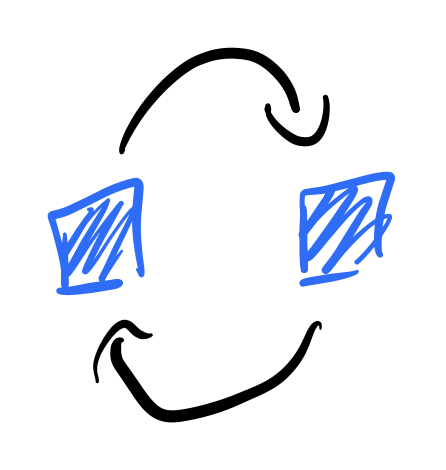
\includegraphics[scale=0.35]{Lectures/Images/lec11-swap.png}
    \end{center}
    \item We can measure $B_1(\gamma)$ for any pair of fluxes:
    \begin{center}
        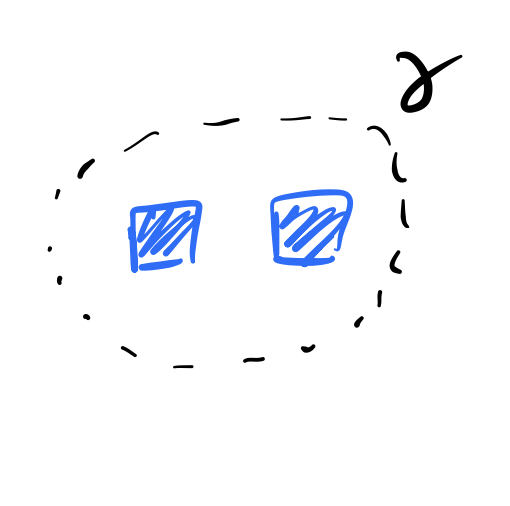
\includegraphics[scale=0.35]{Lectures/Images/lec11-loop.png}
    \end{center}
    Physically, we can measure this by taking charge excitations and braiding them around the loop. So, we could replace this stipulation with the ability to braid charges around fluxes.
    \item We can measure whether a pair of fluxes has trivial total topological charge. For this, we need to braid both charges and fluxes (and both have to be trivial). Physically we could imagine this as some adiabatic evolution.
\end{enumerate}
3 is a subset/coarser measurement than 4. It only measures whether the braid with charges is trivial. 4 measures whether the braid with both charges and fluxes are trivial. Note that we do not need to know \emph{what} the flux is, only whether it is trivial or not.

The claim: If $G$ is a simple (that is, $G$ does not have any nontrivial normal subgroup, where normal means to be preserved under conjugation) non-abelian group, then we can use efficiently simulate (there is a constant overhead to simulate each gate in the universal gateset via braiding) any quantum circuit with these operations.

\begin{center}
    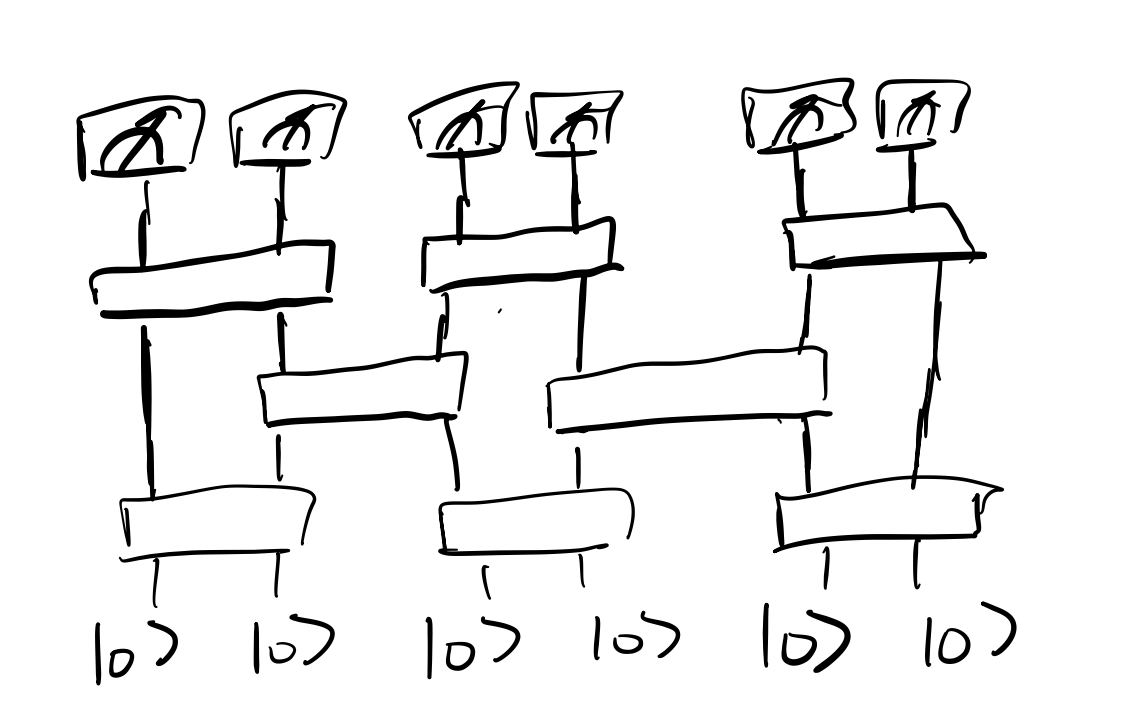
\includegraphics[scale=0.35]{Lectures/Images/lec11-qcircuit.png}
\end{center}

As an example, the smallest simple non-abelian group is $A_5$ (even permutations of 5 elements), with 60 elements. Note that this result has been extended, to smaller groups, e.g. $S_3$.

\subsection{Idea}
Consider $N$ fluxes. 
\begin{center}
    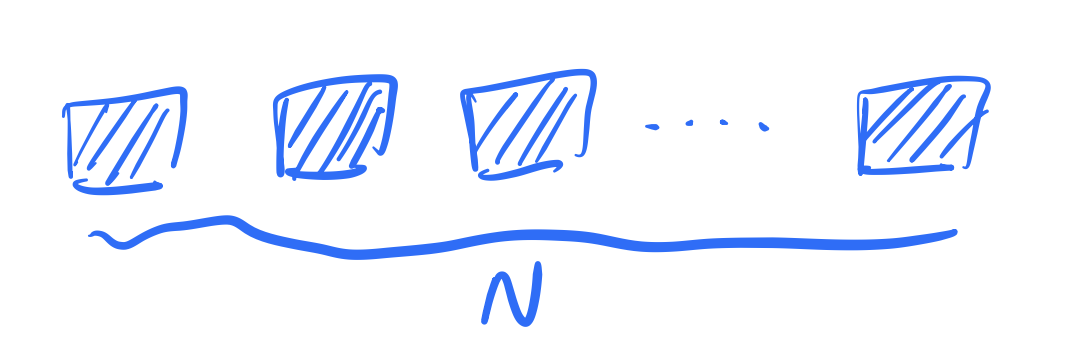
\includegraphics[scale=0.35]{Lectures/Images/lec11-Nfluxes.png}
\end{center}

There is an exponentially large degeneracy $\sim \abs{C}^N$. It turns out that we can define a convenient subspace (sometimes called the computational subspace) of dimension $2^{N/2}$. This allows us to represent $N/2$ qubits. Specifically, choose two elements $a, b \in G$, with $b^2 = 1$ and $ab \neq ba$ (for a non-abelian simple group, we can always find such $a, b$). Define:
\begin{center}
    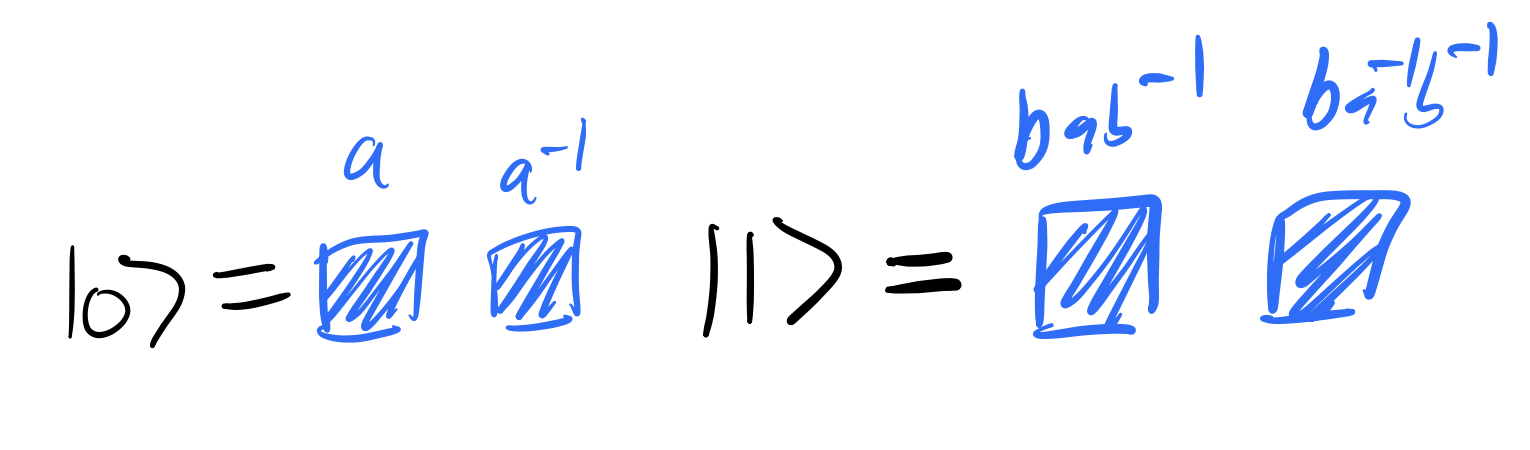
\includegraphics[scale=0.35]{Lectures/Images/lec11-compbasis.png}
\end{center}
A typical computational state (say $\ket{0100\ldots}$) then looks like:
\begin{center}
    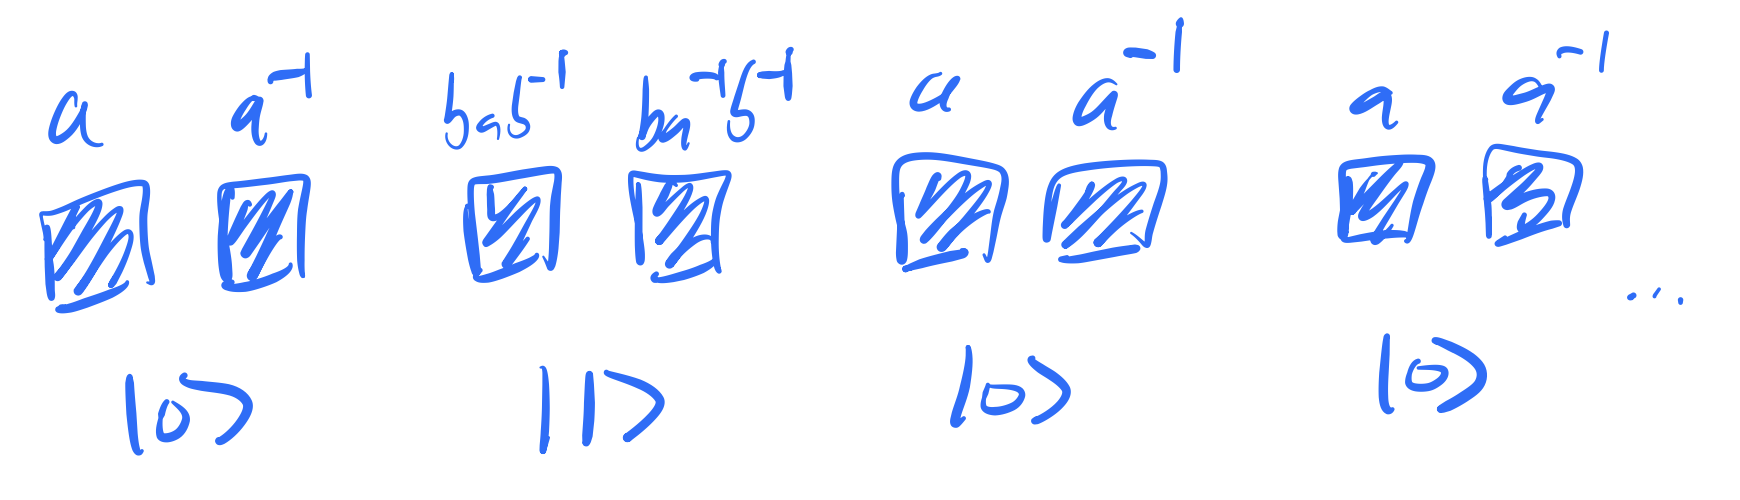
\includegraphics[scale=0.35]{Lectures/Images/lec11-basisstateexample.png}
\end{center}

Note that there are a few ancillary fluxes\footnote{John Preskill calls this the ``flux bureau of standards''.} which fixes the issue of uniform conjugation which maps $\ket{0} \leftrightarrow \ket{1}$ - these ancillary fluxes are the ``reference fluxes'' which allow us to tell apart $\ket{0}$ and $\ket{1}$.

If the group is simple, we can perform the Toffoli gate - a particular 3 qubit gate - using braiding. Note that this is a classical gate universal for classical computation. Further, we can apply and measure single qubit Paulis $X,Y,Z$. 

Measuring $Z$ is simple; if we have a reference flux (say, $a$), we can measure $B_1(\gamma)$ around the reference flux and one half of the pairs of fluxes that make up $\ket{0}$ or $\ket{1}$. For $\ket{0}$ we find the flux is trivial and for $\ket{1}$ we find the flux is nontrivial.

Measuring $X$ has to do with measuring the total topological charge. If we are in the state $\ket{0} - \ket{1}$, we have a state which is orthogonal to the state which has trivial total topological charge, because $\ket{0}, \ket{1}$ have trivial total topological charge, and only a symmetric combination of these will have trivial total topological charge.

Then $\set{\text{Toffoli}, X, Y, Z}$ is a universal gate set for quantum computation, so we are done! For details, see John Preskill's lecture notes on quantum computation (Chapter 9.11) \url{http://theory.caltech.edu/~preskill/ph219/topological.pdf}.

We don't go through the gory details of this particular protocol, but we do comment that one can prove a similar result for many other types of non-Abelian anyons.

What is the advantage of this kind of model of QC? It is naturally protected against decoherence and errors, so long as anyons are far apart during braiding and measurement (and you work at sufficiently low temperature). In some sense, the quantum error correction is already baked in at the hardware level. This comes from the fact that the system is robust to local perturbations.

\subsection{Defining gapped phases of matter}
Thus far, we have been focusing on very specific models. But we may wonder to the extent to which the properties we have seen are general/persistent, e.g. under perturbations. To discuss this, we want to introduce the notion of a gapped phase of matter.

The setting will be qubits on a lattice with local interactions and an energy gap. What do we mean by ``local'' or ``short-range''? The rough definition is that:
\begin{equation}
    H = \sum_r H_r
\end{equation}
where $H_r$ is supported within a finite distance of $r$.

\begin{center}
    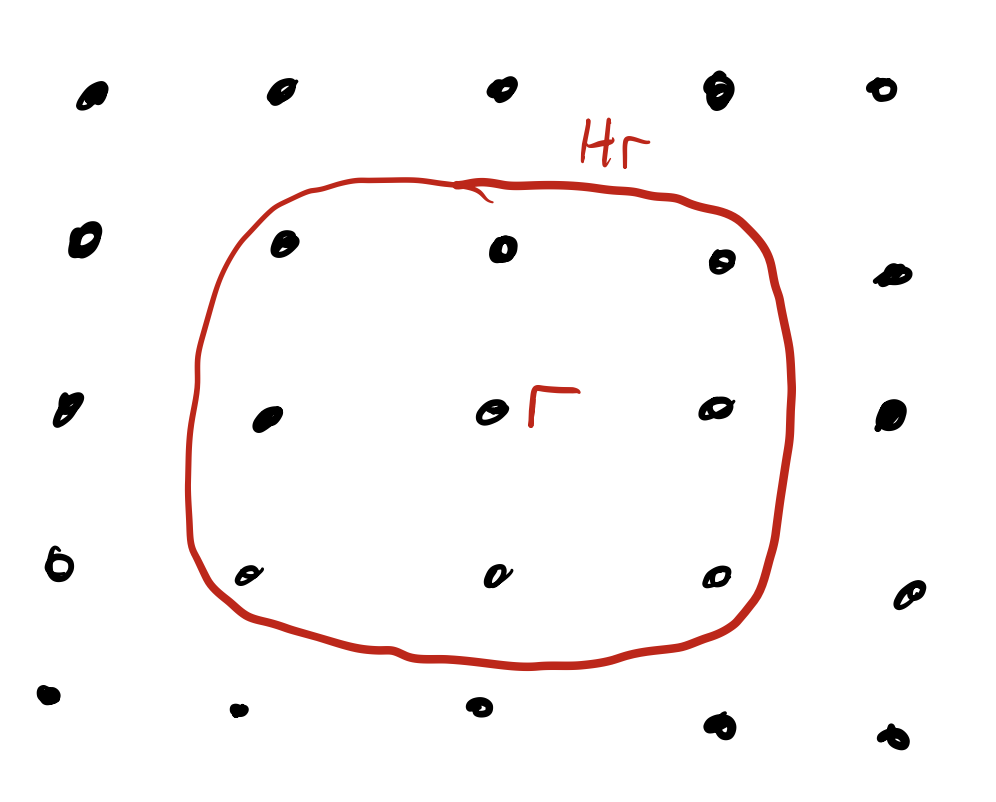
\includegraphics[scale=0.35]{Lectures/Images/lec11-localH.png}
\end{center}

Strictly speaking, we will allow for something slightly more general. Instead of only allowing for strictly short range interactions, we will allow for interactions that decay super-polynomially (faster than any power law):
\begin{equation}
    \norm{[H_r, O_{r'}]} \leq \mathcal{O}(\abs{r - r'}^{-\infty})
\end{equation}
where $\leq \mathcal{O}(\abs{r - r'}^{-\infty})$ means $\leq \frac{C}{\abs{r - r'}^n}$ for any $n$, $O_{r'}$ is some single-site operator at $r'$, and $\norm{\cdot}$ is the operator norm. The classic example is exponentially decaying tails.

By energy gap, we mean that in the thermodynamic limit (system size $\to \infty$) we have a finite energy between the ground state(s) and the excited states of the system.

\textit{Definition.} Two local, gapped Hamiltonians $H_a, H_b$ belong to the same phase if there exists an interpolating family of Hamiltonians $\set{H(s): 0 \leq s \leq 1}$ with $H(0) = H_a, H(1) = H(b)$ such that $H(s)$ is local and gapped for all $s$.

\begin{center}
    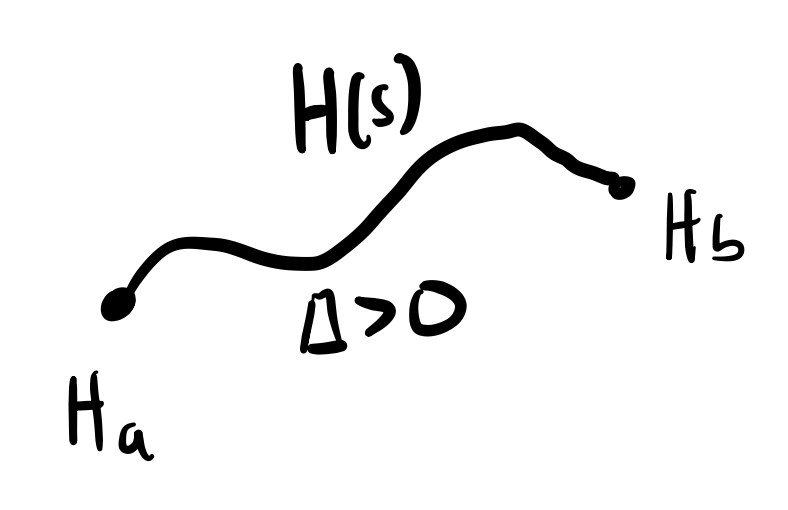
\includegraphics[scale=0.35]{Lectures/Images/lec11-interpolation.png}
\end{center}

Two comments about the definition:
\begin{itemize}
    \item Analogy with the finite $T$ definition of phases. Recall the phase diagram of water:

    Here, two points are in the same phase so long as we can find a path connecting them such that the free energy is smooth/analytic along the path (at the phase transition, we have a non-analyticity). This idea of two points in a phase being connected by a ``nice'' path is analogous.

    \begin{center}
        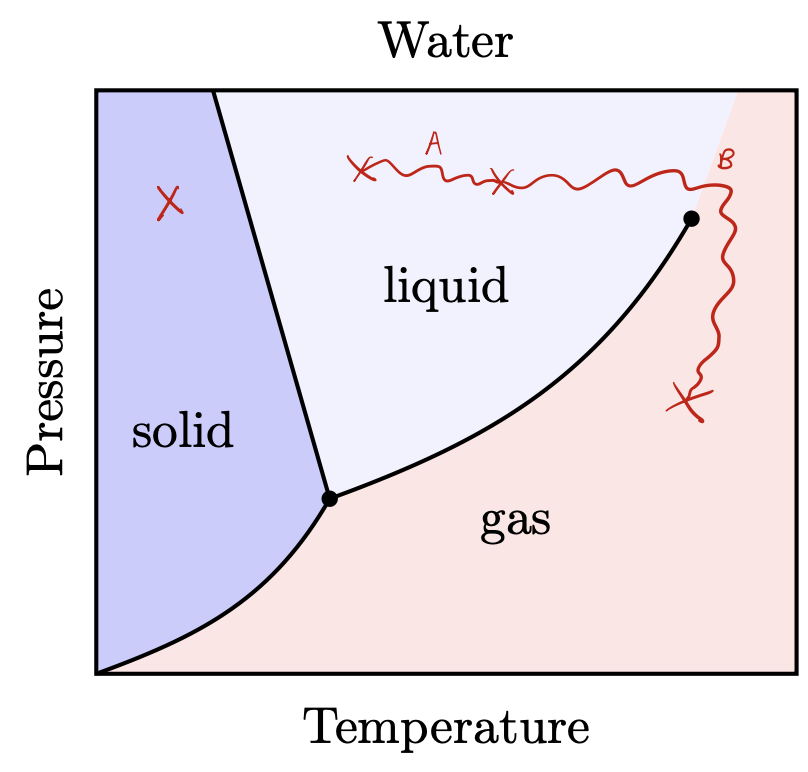
\includegraphics[scale=0.35]{Lectures/Images/lec11-water.png}
    \end{center}

    In the above diagram, two water points are in the same phase (path $A$). Water and steam are also in the same phase, as (going to high enough temperature) we can find a path that smoothly connects water and steam (path $B$). However, there is no path that connects ice with water without going through a phase transition, so these points must correspond to different phases. This points out one condition about the definition - it is easier to conclude that two things are in the same phase (because we need only find a single path that works) vs. things are in different phases (in which case we need to show that \emph{all} paths cannot work).
    \item The existence of an interpolation implies $H_a, H_b$ are adiabatically connected. We thus intuitively expect that $H_a, H_b$ have the same physical properties, since we are able to continuously deform one system into the other.
\end{itemize}
This was the status of phases of matter $> 20$ years ago. But around 2 decades ago, people developed a way to make this intuition more precise, using tools from quantum information.

\subsection{Local Unitary Transformations}
\emph{Definition.} A \emph{local unitary transformation} $U$ is any unitary that can be generated by the time evolution of a local Hamiltonian (with local as we definined previous - either finite range or superpolynomially decaying interactions) over a finite time $t$. In other words, we can write it as the time ordered exponential:
\begin{equation}
    U(T) = \mathcal{T}\exp(-i\int_0^T H(t)dt)
\end{equation}
where $H$ is local.

In what sense is this $U$ local? Generated by something local - certainly, but a priori we cannot measure this. The more physical thing we can measure is the fact that it maps local operators to local operators. This is a result due to Lieb and Robinson.

\textit{Theorem (Lieb-Robinson bound).} Let $U =  \mathcal{T}\exp(-i\int_0^T H(t)dt)$ with $H(t)$ local. Let $O$ be an operator supported in some region $R$. Then, $U^\dag O U$ is supported within distance $v_{LR}T$ of $R$, with superpolynomially decaying tails. $v_{LR}$ is the Lieb-Robinson velocity, and is determined by the range of interactions in $H(t)$.

\begin{center}
    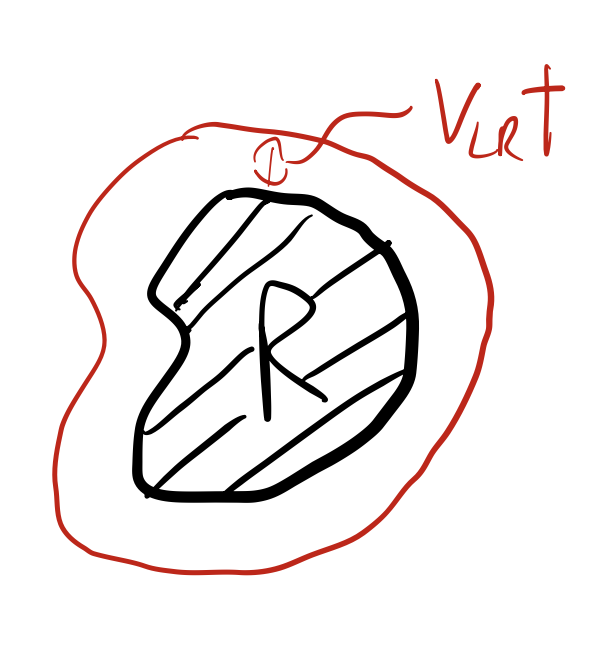
\includegraphics[scale=0.35]{Lectures/Images/lec11-LRbound.png}
\end{center}

Some intuition; if we imagine calculating $U^\dag O U$ for time-independent $H$, we want to calculate something like $e^{iHT}Oe^{-iHT}$. We could then expand this out in a power series:
\begin{equation}
    e^{iHT}Oe^{-iHT} \approx O + iT[H, 0] - \frac{T^2}{2}[H, [H, O]] + \ldots
\end{equation}
wherein if $H$ has short range interactions, each commutator in the power series spreads $O$ slightly.

Next time, we will use these concepts to show that two $H$ in the same phase have ground states that are related by a local unitary transformation.